\documentclass[A4paper,12pt]{report}
\usepackage[centertags]{amsmath}
\usepackage{chapterbib}
\usepackage{amsfonts}
\usepackage{ulem}
\usepackage{amssymb}
\usepackage{tocloft}
\usepackage{multirow}
\usepackage{enumitem}
\usepackage{amsthm}
\usepackage{epsfig}
\usepackage[table,xcdraw]{xcolor}
\usepackage{graphicx}
\usepackage{newlfont}
\usepackage{pdflscape}
\usepackage{hyperref}
\usepackage{mathtools}

\usepackage{ragged2e}
\usepackage{amsmath}
\usepackage{graphicx}
\usepackage{sectsty}
\usepackage{amsmath,latexsym}
\usepackage{amssymb}
\usepackage{etoolbox}
\usepackage{longtable}
\usepackage{tocloft}
\usepackage{setspace}
\usepackage{amsfonts}
\usepackage{amsthm}
\usepackage{float}
\usepackage{epsfig}
\usepackage{epstopdf}
\usepackage{textpos}
\usepackage{placeins}
% for not including: after figure/table number in caption
\usepackage[labelsep=space]{caption}
%\usepackage{caption}
\usepackage{color}
\usepackage{tocloft}
\usepackage{setspace,kantlipsum}
\usepackage[hmargin=1.4in,hmargin=1.4in]{geometry}
\usepackage{mathptmx}
\usepackage{titlesec}
% next 3 lines for reducing space to default before and after section/headings ,etc.
\titlespacing{\section}{0pt}{\parskip}{-\parskip}
\titlespacing{\subsection}{0pt}{\parskip}{-\parskip}
\titlespacing{\subsubsection}{0pt}{\parskip}{-\parskip}

\usepackage{lscape}
\makeatletter
\setlength{\@fptop}{0pt}
\makeatother
\usepackage{booktabs,threeparttable}
\sectionfont{\fontsize{13.5}{15}\selectfont}%                   Faculty of Grad Studies insists on this!?
\subsectionfont{\fontsize{12.5}{15}\selectfont}
\newgeometry{left=1.5in,right=1.0in,top=1in,bottom=1in}
% THEOREMS ---------------------------------------------------------------
\theoremstyle{plain}
\newtheorem{thm}{Theorem}[section]
\newtheorem{cor}[thm]{Corollary}
\newtheorem{lem}[thm]{Lemma}
\newtheorem{Proposition}[thm]{Proposition}
\newtheorem{opn}[thm]{}
\renewcommand\cftchapfont{\fontsize{13}{13}\selectfont\bfseries}
\renewcommand\cftsecfont{\fontsize{13}{13}\selectfont}
\renewcommand\cftsubsecfont{\fontsize{13}{13}\selectfont}
\renewcommand\cftloftitlefont{\fontsize{14.5}{14.5}\selectfont\bfseries}
\renewcommand\cftlottitlefont{\fontsize{14.5}{14.5}\selectfont\bfseries}
\renewcommand\cfttoctitlefont{\fontsize{14.5}{14.5}\selectfont\bfseries}
%\chapternumberfont{\centering\fontsize{17}{17}\selectfont}
%\chaptertitlefont{\centering\fontsize{17}{17}\selectfont\vfill}
%\titleclass{\chapter}{page}
\titleformat{\chapter}[display]{\filcenter\bfseries\fontsize{17}{17}\selectfont}{{\chaptername} \thechapter}{17pt}{}%[\break]%[\vfill]
\titlespacing{\chapter}{0pt}{6ex plus 1fill}{10ex plus 1fill}
\theoremstyle{definition}
\newtheorem{defn}{Definition}[section]
\renewcommand*\listfigurename{\par\hbox{LIST OF FIGURES \strut}\hrule height .05cm}
\renewcommand*\listtablename{\par\hbox{LIST OF TABLES \strut}\hrule height .05cm}
\theoremstyle{remark}
\newtheorem{rem}{Remark}[section]
%\titleformat{\chapter}[display]
%{\normalfont\huge\bfseries\centering}{\centering\chaptertitlename\ \thechapter}{100pt}{\Huge}
%\titlespacing{\chapter}
%{50pt}{50pt}{40pt}
%\renewcommand*{\refname}{} % This will define the headingthe  of bibliography to be empty, so you can...
\renewcommand{\cftpartleader}{\cftdotfill{\cftdotsep}} % for parts
\renewcommand{\cftchapleader}{\cftdotfill{\cftdotsep}} % for chapters
\renewcommand\bibname{}
%for tcontents content, figure, and table pages. setting space before and after
\renewcommand\cftbeforetoctitleskip{0cm}
\renewcommand\cftbeforeloftitleskip{0cm}
\renewcommand\cftbeforelottitleskip{0cm}
\renewcommand\cftaftertoctitleskip{0.5cm}
\renewcommand\cftafterloftitleskip{0.5cm}
\renewcommand\cftafterlottitleskip{0.5cm}
% for having equal length in contentsf content entries (chapters)
%\setlength\cftparskip{-2pt}
\setlength\cftbeforechapskip{0pt}

\numberwithin{equation}{section}
\renewcommand{\theequation}{\thesection.\arabic{equation}}
\renewcommand{\contentsname}{\hfill TABLE OF CONTENTS \hfill}
\titleformat*{\section}{\large\bfseries}
\titleformat*{\subsection}{\fontsize{4.6mm}{4.6mm}\selectfont\bfseries}
\renewcommand*\cftfigpresnum{Fig~}
\settowidth{\cftfignumwidth}{\cftfigpresnum}
\renewcommand{\cftfigaftersnumb}{\quad\quad~}
\newlength\mylen
\settowidth{\mylen}{\cfttabpresnum\cfttabaftersnum}
\addtolength{\cfttabnumwidth}{\mylen}
\setlength\cfttabindent{0pt}
\setlength\cftfigindent{0pt}
\newcolumntype{a}{>{\columncolor{classicrose}}S{p{8.5cm}}}



%for having equalthe  space in list
\makeatletter
%\show\@chapter of table 
\def\@chapter[#1]#2{\ifnum \c@secnumdepth >\m@ne
                         \refstepcounter{chapter}%
                         \typeout{\@chapapp\space\thechapter.}%
                         \addcontentsline{toc}{chapter}%
                                   {\protect\numberline{\thechapter}#1}%
                    \else
                      \addcontentsline{toc}{chapter}{#1}%
                    \fi
                    \chaptermark{#1}%
%                    \addtocontents{lof}{\protect\addvspace{10\p@}}% 
%                    \addtocontents{lot}{\protect\addvspace{10\p@}}%
                    \if@twocolumn
                      \@topnewpage[\@makechapterhead{#2}]%
                    \else
                      \@makechapterhead{#2}%
                      \@afterheading
                    \fi}
\makeatother

%for having equal space in references
\let\oldthebibliography\thebibliography
\let\endoldthebibliography\endthebibliography
\renewenvironment{thebibliography}[1]{
  \begin{oldthebibliography}{#1}
    \setlength{\itemsep}{0em}
   % \setlength{\parskip}{0em}
}
{
  \end{oldthebibliography}
}



\begin{document}
\pagenumbering{roman}
\thispagestyle{empty}
\begin{center}
\onehalfspacing
\Huge{\textbf{Smart Travel Planner}} \\[0.1in]


\includegraphics[width=5cm, height=5cm]{comsats} \\[0.2in]

\textit{\large By} \\[0.2in]

\Large
Malaika Wasiq \\
CIIT/SP23-BSE-041/ATK \\[0.2in]
Amima Masood \\
CIIT/SP23-BSE-038/ATK \\[0.25in]

Project \\[0.25in]
for \\[0.25in]

\Large{Bachelor of Science in Software Engineering} \\[0.4in]

\LARGE
COMSATS University Islamabad \\
Attock Campus - Pakistan \\[0.3in]

\Large{December, 2026}
\end{center}


\clearpage
\newpage
\hspace{-5em}\raisebox{-1\baselineskip}{
\includegraphics[width=3cm, height=3cm]{comsats}}
\begin{tabular}[b]{l}
\vspace{.75cm}
  \Large{\textbf{COMSATS University Islamabad, Attock Campus}}\\
\end{tabular}
\hfill
\begin{center}
\vspace{0.1in}
\onehalfspacing\LARGE{\textbf{Smart Travel Planner}} \\
\vspace{0.5in}
\large{This Project is Presented to}\\
\vspace{0.5in}
\Large{COMSATS University Islamabad Attock Campus}\\
\vspace{0.5in}
\large{In partial fulfillment\\
\vspace{0.1in}
of the requirement for the degree of}\\
\vspace{0.5in}
\LARGE{BS in Software Engineering}\\
\vspace{0.4in}
\normalsize{By}\\
\vspace{0.3in}
\large{Malaika Wasiq\\
CIIT/SP23-BSE-041/ATK}\\[0.15in]
\large{Amima Masood\\
CIIT/SP23-BSE-038/ATK}\\
\vspace{0.4in}
\Large{December, 2026}
\end{center}


\newpage
\begin{center}
\onehalfspacing\LARGE \uline{\textbf{Smart Travel Planner}}\\
\end{center}
\vspace{0.2in}

\onehalfspacing\noindent\large{This final year project is submitted to the Department of Computer Science as partial fulfillment of the requirements for the award of the degree of BS in Software Engineering.}
\vspace{0.4in}
\begin{table}[ht!]
\centering
{\setlength{\arrayrulewidth}{0.7mm}
\setlength{\tabcolsep}{45pt}
\renewcommand{\arraystretch}{2.2}
\begin{tabular}{|c|c|}
\hline
\rowcolor[HTML]{656565}
 \large{\textbf{\textcolor{white}{Name}}} &\large{\textbf{\textcolor{white}{Registration Number}}}  \\
 \hline
 Malaika Wasiq & CIIT/SP23-BSE-041/ATK \\ \hline
 Amima Masood & CIIT/SP23-BSE-038/ATK \\ \hline
\end{tabular}
}
\end{table}
\FloatBarrier
\vspace{1.5in}

\noindent\large{\textbf{Supervisor}}
\begin{flushleft}
\vspace{0.2in}
\large{Mr. Muhammad Waseem Khan\\
\vspace{0.1in}
Lecturer,\\
Department of Computer Science\\
\vspace{0.1in}
COMSATS University Islamabad, Attock Campus\\

\vspace{0.2in}
December, 2026 }
\end{flushleft}



\newpage
\begin{center}
\Large{\textbf{{Final Approval}}}
\par\noindent\rule{\textwidth}{0.6pt}
\end{center}

\begin{center}
\normalsize {This Project titled}\\
\vspace{0.05in}
\LARGE{\textbf{Smart Travel Planner}}\\
\vspace{0.4in}

\normalsize{By}\\
\vspace{0.3in}
\large{\textit{Malaika Wasiq}\\
{\textit{CIIT/SP23-BSE-041/ATK}}}\\[0.15in]
\large{\textit{Amima Masood}\\
{\textit{CIIT/SP23-BSE-038/ATK}}}\\
\vspace{0.4in}

\normalsize{Has been approved for the COMSATS University Islamabad, Attock Campus.}\\
\end{center}

\vspace{0.1in}
\noindent External Examiner:\line(1,0){260}
\begin{center}
\normalsize{External Examiner \\
University Name}\\
\end{center}
\vspace{0.1in}
Supervisor:\line(1,0){310}
\begin{center}
\normalsize{Mr. Muhammad Waseem Khan\\
Lecturer, Department of Computer Science, (CUI) Attock Campus}
\end{center}
\vspace{0.1in}
HoD:\line(1,0){345}
\begin{center}
\normalsize{Dr. Muazzam Maqsood\\
Associate Professor, Department of Computer Science, (CUI) Attock Campus}
\end{center}

\begin{spacing}{1.5}
\newpage
\begin{center}
\Large{\textbf{\underline {Author’s Declaration}}}\\
\end{center}

\noindent\normalsize{We, ``Malaika Wasiq'' (CIIT/SP23-BSE-041/ATK) and ``Amima Masood'' (CIIT/SP23-BSE-038/ATK), hereby declare that we have produced the work presented in this project, during the scheduled period of study. We also declare that we have not taken any material from any source except in reference to where that amount of plagiarism is within an acceptable range. If a violation of HEC rules on research has occurred in this thesis, we shall be liable to punishable action under the plagiarism rules of HEC.}\\

\vspace{0.8in}
\begin{flushright}
Student Signature: \line(1,0){120}\\
\vspace{0.05in}
\textbf{Malaika Wasiq}\\
CIIT/SP23-BSE-041/ATK
\end{flushright}

\vspace{0.4in}
\begin{flushright}
Student Signature: \line(1,0){120}\\
\vspace{0.05in}
\textbf{Amima Masood}\\
CIIT/SP23-BSE-038/ATK
\end{flushright}

\vspace{0.2in}
Date:\line(1,0){100}\hfill
\end{spacing}

\newpage
\begin{center}
\Large{\textbf{\underline {Certificate}}}\\
\vspace{0in}
\end{center}
It is certified that ``Malaika Wasiq'' (CIIT/SP23-BSE-041/ATK) and ``Amima Masood'' (CIIT/SP23-BSE-038/ATK) have carried out all the work related to this project under my supervision at the Department of Computer Science, COMSATS University Islamabad, Attock Campus, and the work fulfills the requirements for the award of the degree of BS in Software Engineering.\\
\vspace{0.5in}
\begin{flushright}
\begin{tabular}{@{}r@{}}
Supervisor\\
\vspace{0.3in}
\line(2,0){120}\\
Mr. Muhammad Waseem Khan\\
Lecturer,\\
Department of Computer Science,\\
CUI, Attock Campus
\end{tabular}
\end{flushright}

\begin{flushleft}
Head of Department:\\
\vspace{0.2in}

\line(1,0){100}\\
\vspace{0.2in}
Dr. Muazzam Maqsood\\
Associate Professor,\\
Department of Computer Science,\\
CUI, Attock Campus
\end{flushleft}


\newpage
\thispagestyle{empty}
\begin{center}
\vspace*{\fill}
\begin{spacing}{1.5}
\Large\textit{Dedicated to our parents,\\
    who have always been our biggest supporters\\
    and a constant source of inspiration}
\end{spacing}
\vspace*{\fill}
\end{center}


\newpage
\begin{center}
\Large\textbf{{ACKNOWLEDGEMENTS}}\\
\end{center}
\vspace{0.2in}
\begin{center}
\textbf{Praise to be ALLAH, the Cherisher and Lord\\of the World, Most gracious and Most Merciful}
\end{center}
\vspace{0.2in}
\begin{spacing}{1.5}
\justify\noindent \normalsize{We would like to express our deepest gratitude to Allah Almighty for giving us the strength, knowledge, and patience to complete this project successfully. We are sincerely thankful to our supervisor, Mr. Muhammad Waseem Khan, for his continuous guidance, valuable feedback, and encouragement throughout the development of this project. His support played a key role in shaping the direction and quality of our work. We would also like to thank the faculty members of the Department of Computer Science at COMSATS University Islamabad, Attock Campus, for their teaching and support during our academic journey. Their knowledge and dedication have greatly contributed to our learning and growth. A special thanks to our families and friends for their unconditional love, patience, and moral support throughout our studies. Their belief in us kept us motivated during difficult times. Finally, we would like to acknowledge all the researchers and developers whose work and open source tools provided a strong foundation for this project.}

\begin{flushright}
\vspace{0.4in}
Malaika Wasiq\\
CIIT/SP23-BSE-041/ATK\\[0.15in]
Amima Masood\\
CIIT/SP23-BSE-038/ATK
\end{flushright}
\end{spacing}

\newpage
\begin{center}
\Large{\textbf{Project Summary}}\\
\end{center}
\setlength{\parindent}{0pt}
\begin{spacing}{1.5}
\normalsize{Planning a trip can often be stressful and time-consuming because travelers have to switch between many different apps and websites to find attractions, check weather forecasts, estimate budgets, and book hotels. Many existing travel tools offer generic suggestions that do not take into account individual preferences, financial limitations, or daily schedules. 

The Smart Travel Planner is a mobile and web software system designed to simplify trip organization. The system brings all necessary travel planning features into a single, unified application. Users can create customized daily itineraries based on their selected destination, travel dates, and budget limits. The application integrates real-time weather information to ensure that suggested activities match the forecasted weather conditions. It also provides interactive map routing to help travelers visualize their daily journeys and minimize travel time. In addition, the system includes hotel recommendations, budget tracking with expense categorization, and an interactive assistant to answer travel questions. 

By combining itinerary generation, map navigation, budget tracking, and destination insights into one easy-to-use platform, the Smart Travel Planner reduces planning effort and helps travelers enjoy a well-organized travel experience.}
\end{spacing}
\begin{spacing}{1.5}
\newpage
\renewcommand{\cftaftertoctitle}{\hfill}
\renewcommand*\cftaftertoctitle{{\strut \hfill}\hrule height .05cm}
%\setlength\cftparskip{0pt}
%\setlength\cftbeforechapskip{0pt}

\!
\tableofcontents
\!

\!
\centering \renewcommand*\listfigurename{LIST OF FIGURES}
\renewcommand{\cftafterloftitle}{\hfill}
\renewcommand*\cftafterloftitle{{\strut \hfill}\hrule height .05cm}
% Center the title of the list of figures on a separate line
\newpage
\listoffigures
\!
\clearpage
{\let\oldnumberline\numberline%
\renewcommand{\numberline}{\tablename~\oldnumberline}%
\centering \renewcommand*\listtablename{LIST OF TABLES}
\renewcommand{\cftafterlottitle}{\hfill}
\renewcommand*\cftafterlottitle{{\strut \hfill}\hrule height .05cm}
\listoftables}
\clearpage
\end{spacing}


\begin{spacing}{1.5}
\pagenumbering{arabic}% Arabic page numbers (and reset to 1)
\chapter{Introduction}
\thispagestyle{empty}
\newpage
%\noindent
\setlength{\parindent}{0pt}
\end{spacing}

\begin{spacing}{1.5}
\pagenumbering{arabic}

\thispagestyle{empty}

% --- Centered chapter title, same size as normal chapter ---
{\centering \Large \bfseries Chapter Overview \par}
\vspace{1cm} % adjust space after title

% --- Chapter introduction text (not numbered) ---
This chapter introduces the background, motivation, and problem
statement of the project. It highlights the research gap and explains
why this study is important. The chapter also outlines the objectives
and structure of the work.

\end{spacing}


\section{Introduction}
Lorem ipsum dolor sit amet, consectetuer adipiscing elit. Maecenas porttitor congue massa. Fusce posuere, magna sed pulvinar ultricies, purus lectus malesuada libero, sit amet commodo magna eros quis urna. Nunc viverra imperdiet enim. Fusce est. Vivamus a tellus. Pellentesque habitant morbi tristique senectus et netus et malesuada fames ac turpis egestas. Proin pharetra nonummy pede. Mauris et orci. Aenean nec lorem. In porttitor. Donec laoreet nonummy augue. Suspendisse dui purus, scelerisque at, vulputate vitae, pretium mattis, nunc. Mauris eget neque at sem venenatis eleifend. Ut nonummy. Fusce aliquet pede non pede. Suspendisse dapibus lorem pellentesque magna. Integer nulla. Donec blandit feugiat ligula. Donec hendrerit, felis et imperdiet euismod, purus ipsum pretium metus, in lacinia nulla nisl eget sapien.\ref{fig:fig1.1} shows different biometric features.






By comparing the derived model parameters, gait recognition systems can identify individuals based on the unique characteristics of their gait models. Model-based approaches use body parameters as features hence also needing high-resolution videos \cite{P}. Overall, model-based gait recognition offers a comprehensive and detailed analysis of gait patterns by incorporating mathematical models. This approach provides valuable insights into the underlying biomechanics of gait and has the potential to improve recognition accuracy in gait recognition systems.

\section{Significance of the Proposed System}
Write a concise vision statement that summarizes the long-term purpose, intent and significance of the product. The vision statement should reflect a balanced view that will satisfy the expectations of diverse stakeholders. It can be somewhat idealistic but should be grounded in the realities of existing or anticipated markets. The following keyword template works well for crafting a product vision statement:

\textbf{For} [target customer]

\textbf{Who} [statement of the need or opportunity]

\textbf{The} [product name]

\textbf{Is} [product category]

\textbf{That} [major capabilities, key benefit, compelling reason to buy or use]

\textbf{Unlike} [primary competitive alternative, current system, current business process]

\textbf{Our product} [statement of primary differentiation and advantages of new product]

Here’s a sample vision statement for the Chemical Tracking System, with the keywords in boldface:

\textit{\textbf{For} employees \textbf{who} want to order meals from the company cafeteria or from local restaurants online, \textbf{the} Cafeteria Ordering System is an Internet-based and smartphone-enabled application \textbf{that} will accept individual or group meal orders, process payments, and trigger delivery of the prepared meals to a designated location on the Process Impact campus. \textbf{Unlike} the current telephone and manual ordering processes, employees who use \textbf{our product} (the Cafeteria Ordering System) will not have to go to the cafeteria to get their meals, which will save them time and will increase the food choices available to them.}


This chapter discusses the precise problem to be solved. It should extend to include the outcome.

\section{Problem Statement}

Provide a problem statement in a concise paragraph describing 

\textbf{Why} are you developing this software system? 

\textbf{What} problem your software system is going to solve?

[Usually in 10-16 sentences]

\textbf{Example:}

\textit{Employees at the company Process Impact presently spend an average of 65 minutes per day going to the cafeteria to select, purchase, and eat lunch. About 20 minutes of this time is spent walking to and from the cafeteria, selecting their meals, and paying by cash or credit card. When employees go out for lunch, they spend an average of 90 minutes off-site. Some employees phone the cafeteria in advance to order a meal to be ready for them to pick up. Employees don‘t always pet the selections they want because the cafeteria runs out of certain items. The cafeteria wastes a significant quantity of food that is not purchased and must be thrown away. These same issues apply to breakfast and supper, although far fewer employees use the cafeteria for those meals than for lunch.}

\section{Scope and Objectives}
Write down the scope of your project in a paragraph. Briefly define the main functionalities of the proposed project. Scope defines the boundaries and range of the proposed solution, that what would be the part of your project. Write down in logical flow with consistency. 
(Usually in 14-18 sentences)

The objectives of our proposed system our three fold. 
% replace the word three with the number of the objectives

\newlength{\desclabelwidth} 
\settowidth{\desclabelwidth}{\textbf{PO1}}
\addtolength{\desclabelwidth}{\labelsep}
\textbf{Example:}
\begin{description}[noitemsep,nolistsep,leftmargin=2cm]
    \item[PO1] Reduce the cost of cafeteria food wastage by 40\%.
    \item[PO2] Reduce cafeteria operating costs by 15%.
    \item[PO3] Increase average effective work time by 15 minutes per cafeteria-using employee per day.
\end{description}


\section{System Limitations/Constraints}
Write down the limitations and constraints of the proposed project. 

Example:

%\newlength{\desclabelwidth} 
%\settowidth{\desclabelwidth}{\textbf{L1}}
%\addtolength{\desclabelwidth}{\labelsep}
\begin{description}[noitemsep,nolistsep,leftmargin=2cm]
	\item [L1] Some food items that are available from the cafeteria will not be suitable for delivery, so the delivery menus available to patrons of the COS must be a subset of the full cafeteria menus. 
	\item [L2] The COS shall be used only for the cafeteria at the Process Impact campus in Clackamas, Oregon. 
\end{description}


\section{Project Deliverables}
List down the project deliverables briefly.
\begin{itemize}
	\item deliverable 1
	\item deliverable 2
\end{itemize}



\section{Relevance to Course Modules}
A brief explanation of how your project is related to various courses studied during BCS.



\section{ Contribution }

This study proposes a novel deep learning framework, which utilizes parallel running custom kernels in order to extract dynamic and static feature maps from the input GEI image. 



\section{ Chapter Summary }

The chapter begins by providing an introduction to gait analysis, highlighting its practical applications in real-life scenarios. It then transitions to the various methods utilized for gait recognition. Section 1.1 delves into Appearance-based methods, while section 1.2 focuses on model-based approaches. The subsequent section sheds light on covariate conditions in gait analysis and their impact. Following that, sections 1.4 and 1.5 address the problem statement and research objectives respectively. Lastly, the chapter concludes by discussing the hypothesis proposed as a potential solution to the identified problem.


\chapter{Literature Review}
\thispagestyle{empty}
\newpage
\begin{spacing}{1.5}
\pagenumbering{arabic}

\thispagestyle{empty}

% --- Centered chapter title, same size as normal chapter ---
{\centering \Large \bfseries Chapter Overview \par}
\vspace{1cm} % adjust space after title

% --- Chapter introduction text (not numbered) ---
This chapter introduces the ...........
There are different methods based on which Gait analysis has been done in past and can be classified into three types of approaches.

\end{spacing}


\section{Write first Application problem details or research papers}

The problem of known and unknown covariates was tackled by using a simple CNN model for known covariates and employing discriminative and Multi-layer Perceptron as classifiers for unknown covariates \cite{4}. A Gaussian Process classification (GP) architecture was proposed to approximate the viewpoint of each probe gait sequence. At various view angles, gait sequences were captured, and then to measure the similarity between them, Canonical Correlation Analysis (CCA) was used to design the correlation of gait sequences from multiple viewpoints while correlation strength was used as a similarity measure \cite{5}. 

\section{Write second Application problem details or research papers}

Shiraga et al, \cite{11} introduced a network model known as GEInet function. A similar approach was used in \cite{12} which used multiple pooling and convolution layers to extract gait templates \cite{13}, which used a framework (TS-CNN) consisting of two-stream CNN architecture which matches mid-level features by learning \cite{14}. Transfer learning uses knowledge from already learned networks, where \cite{15} proposed a framework that used transfer  \cite{16} which was prone to noise in sensory .
\section{Model-Based Methods}

A gait recognition approach was introduced in \cite{19}, also known  \cite{ao} examined three different gait conditions: normal gait, simulated leg length difference, and simulated leg weight difference. Kinematic temporal changes during gait were captured using an online motion recording system. 
A gait recognition approach was introduced in \cite{19}, also known  \cite{ao} examined three different gait conditions: normal gait, simulated leg length difference, and simulated leg weight difference. Kinematic temporal changes during gait were captured using an online motion recording system. 
\begin{table}[h!]
\centering
\caption{Related System Analysis with proposed project solution}
\label{tab:sample}
\begin{tabular}{|p{0.3\textwidth}|p{0.3\textwidth}|p{0.3\textwidth}|}
\hline
\textbf{Application Name} & \textbf{Weakness} & \textbf{Proposed Project Solu
tion} \\ \hline
Row 1, Cell 1 & Row 1, Cell 2 & Row 1, Cell 3 \\ \hline
Row 2, Cell 1 & Row 2, Cell 2 & Row 2, Cell 3 \\ \hline
Row 3, Cell 1 & Row 3, Cell 2 & Row 3, Cell 3 \\ \hline
Row 4, Cell 1 & Row 4, Cell 2 & Row 4, Cell 3 \\ \hline
Row 5, Cell 1 & Row 5, Cell 2 & Row 5, Cell 3 \\ \hline
\end{tabular}
\end{table}




\section{Chapter Summary}

Chapter sumamry comes here

\chapter{Requirement Analysis}
% for hiding page number
\thispagestyle{empty}
\newpage
\begin{spacing}{1.5}
\pagenumbering{arabic}

\thispagestyle{empty}

% --- Centered chapter title, same size as normal chapter ---
{\centering \Large \bfseries Chapter Overview \par}
\vspace{1cm} % adjust space after title

% --- Chapter introduction text (not numbered) ---
This chapter introduces the background, motivation, and problem
statement of the project. It highlights the research gap and explains
why this study is important. The chapter also outlines the objectives
and structure of the work.

\end{spacing}
\section{User classes and characteristics}
Identify the various user classes that you anticipate will use this product, and describe their pertinent characteristics. \textcolor{red}{\textit{See Appendix A of the word document for an example of how to present user classes and characteristics.}}
\section{Requirement Identifying Technique}
This section describes the requirements identifying technique(s) which further help to derive functional requirements specification. The selection of the technique(s) will depend on the type of project. For instance,

\begin{itemize}
	\item Use case (use case diagram + detail use case) is an effective technique for interactive end-user applications.
	\item Event- response table is for real-time system in which most of the functionalities are performed at backend.
	\item Storyboarding for graphically intensive applications. 
\end{itemize}



\section{Functional Requirements}

This section describes the FR of the system expressed in the natural language style. This section is typically organized by feature as a system feature name and specific functional requirements associated with this feature. It is just one possible way to arrange them. Other organizational options include arranging functional requirements by use case, process flow, mode of operation, user class, stimulus, and response depend on what kind of technique has been used to understand functional requirements. Hierarchical combinations of these elements are also possible, such as use cases within user classes. For further detail see Chapter 10 “Documenting the requirements”. Let consider the feature scheme as an example.


\subsection{Functional Requirement X}
Itemize the specific functional requirements associated with each feature. These are the software capabilities that must be implemented for the user to carry out the feature’s services or to perform a use case. Describe how the product should respond to anticipated error conditions and to invalid inputs and actions. Uniquely label each functional requirement, as described earlier. You can create multiple attributes for each functional requirement, such as rationale, source, dependencies, etc. The following template is required to write functional requirements. For further detail see Chapter 11” Writing excellent requirements”.

\begin{table}[t]
	\centering
	\caption{Description of FR-1 - A multi row table}
	\begin{tabular}[c]{|p{4cm}|p{10cm}|}
		\toprule
		\textbf{Identifier} &\textbf{FR-1}\\
		\midrule
		\textbf{Title} & Title of Requirement \\
		\midrule
		\textbf{Requirement}&Description of requirement which may be written either from the user or system perspective e.g. \linebreak
		If written in a \textbf{user perspective:} The [user class or actor name] shall be able to [do something] [to some object] [qualifying conditions, response time, or quality statement].\linebreak
		If written in a \textbf{system perspective:} [optional precondition] [optional trigger event] the system shall [expected system response] \\
		\midrule
		\textbf{Source} & Where this requirement comes from (who originate it)\\
		\midrule
		\textbf{Rationale} & The motivation behind the requirement \\
		\midrule
		\textbf{Business Rule (if required)} & Any restriction, policy, the rule that the particular requirement must be fulfilled through its functional behavior\\
		\midrule
		\textbf{Dependencies} & Requirements ID that is dependent on this requirement \\
		\midrule
		\textbf{Priority} & High / Medium / Low\\
		\bottomrule
		
		
	\end{tabular}
\end{table}

\section{Non-Functional Requirements}
This section specifies nonfunctional requirements other than constraints, which are recorded in section 2.3, and external interface requirements, which will appear in section 7. These quality requirements should be specific, quantitative, and verifiable. Chapter 14 “beyond functionality” presents more information about these quality attribute requirements and many examples. The following are some examples of documenting guidelines.
\subsection{Reliability} 
Requirements about how often the software fails. The measurement is often expressed in MTBF (mean time between failures). The definition of a failure must be clear. Also, don't confuse reliability with availability which is quite a different kind of requirement.  Be sure to specify the consequences of software failure, how to protect from failure, a strategy for error detection, and a strategy for correction.
\subsection{Usability}
Usability requirements deal with ease of learning, ease of use, error avoidance and recovery, the efficiency of interactions, and accessibility. The usability requirements specified here will help the user interface designer create the optimum user experience.
Example:

USE-1: The COS shall allow a user to retrieve the previous meal ordered with a single interaction.

\subsection{Performance}
State specific performance requirements for various system operations. If different functional requirements or features have different performance requirements, it’s appropriate to specify those performance goals right with the corresponding functional requirements, rather than collecting them in this section. 
Example:

PER-1:	 95\% of webpages generated by the COS shall download completely within 4 seconds from the time the user requests the page over a 20 Mbps or faster Internet connection.

\subsection{Security} 
One or more requirements about protection of your system and its data. The measurement can be expressed in a variety of ways (effort, skill level, and time) to break into the system.  Do not discuss solutions (e.g. passwords) in a requirements document.

\section{External Interface Requirements}
This section provides information to ensure that the system will communicate properly with users and with external hardware or software elements. A complex system with multiple subcomponents should create a separate interface specification or system architecture specification. The interface documentation could incorporate material from other documents by reference. For instance, it could point to a hardware device manual that lists the error codes that the device could send to the software. 

\subsection{User Interfaces Requirements}
Describe the logical characteristics of each user interface that the system needs. Some possible items to include are

\begin{itemize}
	\item References to GUI standards or product family style guides that are to be followed.
	\item	Standards for fonts, icons, button labels, images, color schemes, field tabbing sequences, commonly used controls, and the like.
	\item	Screen layout or resolution constraints.
	\item	Standard buttons, functions, or navigation links that will appear on every screen, such as a help button.
	\item	Shortcut keys.
	\item	Message display conventions.
	\item	Layout standards to facilitate software localization.
	\item	Accommodations for visually impaired users.	
\end{itemize}

Document the user interface design details, such as specific dialog box layouts, in a separate user interface specification, not in the SRS . Including screen mock-ups in the SRS  to communicate another view of the requirements is helpful but make it clear that the mock-ups are not the committed screen designs. If the SRS is specifying an enhancement to an existing system, it sometimes makes sense to include screen displays exactly as they are to be implemented. The developers are already constrained by the current reality of the existing system, so it's possible to know up front just what the modified, and perhaps the new, screens should look like.  

\subsection{Software interfaces}
Describe the connections between this product and other software components (identified by name and version), including other applications, databases, operating systems, tools, libraries, websites, and integrated commercial components (If any).
Example:

SI-1: Cafeteria Inventory System
SI-1.1:	The COS shall transmit the quantities of food items ordered to the Cafeteria Inventory System through a programmatic interface.

\subsection{Hardware interfaces}
Describe the characteristics of each interface between the software components and hardware components, if any, of the system. This description might include the supported device types, the data and control interactions between the software and the hardware, and the communication protocols to be used. For more about specifying requirements for systems containing hardware, see Chapter 26, “Embedded and other real-time systems projects.”

\subsection{Communications interfaces}
State the requirements for any communication functions the product will use, including email, web browser, network protocols, and electronic forms.

Example:

CI-1:	The COS shall send an email or text message (based on user account settings) to the Patron to confirm acceptance of an order, price, and delivery instructions.





\section{Chapter Summary}


\chapter{Design and Architecture
}
\thispagestyle{empty}
\newpage
\begin{spacing}{1.5}
\pagenumbering{arabic}

\thispagestyle{empty}

% --- Centered chapter title, same size as normal chapter ---
{\centering \Large \bfseries Chapter Overview \par}
\vspace{1cm} % adjust space after title

% --- Chapter introduction text (not numbered) ---
This chapter introduces the background, motivation, and problem
statement of the project. It highlights the research gap and explains
why this study is important. The chapter also outlines the objectives
and structure of the work.

\end{spacing}

\section{Modules}
Write down the modules of the proposed project.   
Each module should highlight features, using bulleted/numbered notation. 
When developing both a mobile app and a web app, group the modules according to the system types, such as, Client Web App, Client Mobile App, Admin Web App etc.


\subsection{Module 1:  Module Name and Description}
\begin{description}
\item[FE1] Order and pay for meals from the cafeteria menu to be picked up or delivered. 
	
	\item[FE2] Order and pay for meals from local restaurants to be delivered.
\end{description}


\textbf{\textcolor{red}{You add more module if you required}}




\section{Architectural Design}
Develop a modular program structure and explain the relationships between the modules to achieve the complete functionality of the system. This is a high-level overview of how the system’s modules collaborate with each other in order to achieve the desired functionality.

Don’t go into too much detail about the individual subsystems. The main purpose is to gain a general understanding of how and why the system was decomposed, and how the individual parts work together. 

Provide a diagram showing the major subsystems and their connections \ref{architecture}. 

\begin{itemize}
	\item In initial design stage create Box and Line Diagram for simpler representation of the systems
	\item After finalizing architecture style/pattern diagram (MVC, Client-Server, Layered, Multi-tiered) create a detailed mapping modules/components to each part of the architecture
\end{itemize}

\textcolor{red}{\textit{To view example of box and line diagram and architecture styles, see Appendix B. One more thing if your image is not set in relevnt place you can change dimesnion of your images in this code . change the image code parameter instead of image.}}

\begin{figure}[h]
	\centering
	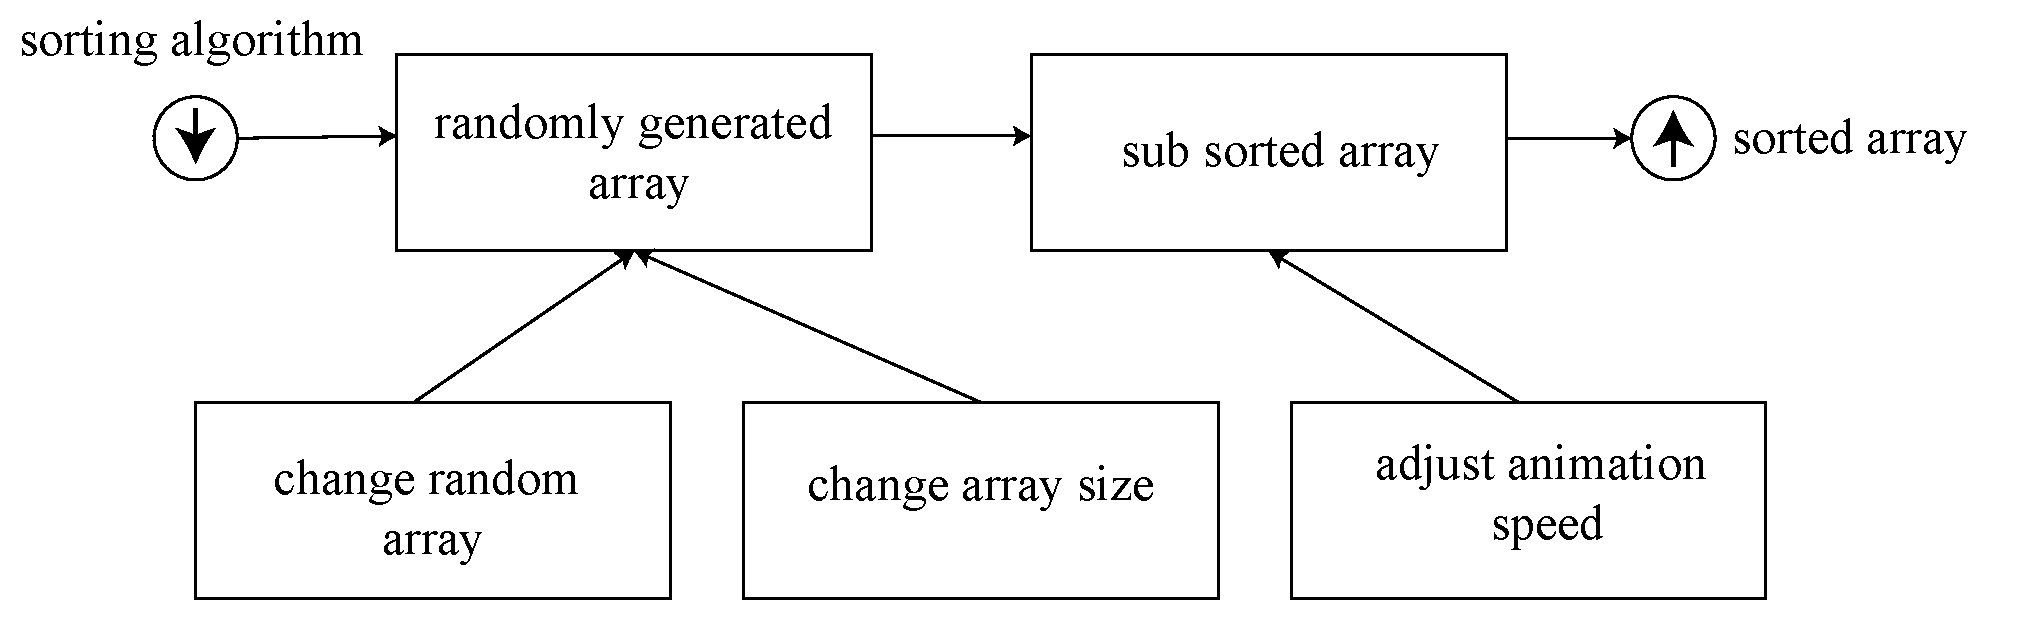
\includegraphics[width=\linewidth]{architecture.pdf}
	\caption{A sample architecture diagram}
	\label{architecture}
\end{figure}
\newpage

\section{Design Models}
Create design models as are applicable to your system. Provide detailed descriptions with each of the models that you add. Also ensure visibility of all diagrams. 


\subsection{Activity Diagram}
\subsubsection{Activity Diagram}
This section describes the Activity Diagram also add diagrma .






\subsection{Usecase Diagram}
Add description and diagram


\subsection{Class Diagram}
Add description and diagram
\begin{figure}[h]
    \centering
    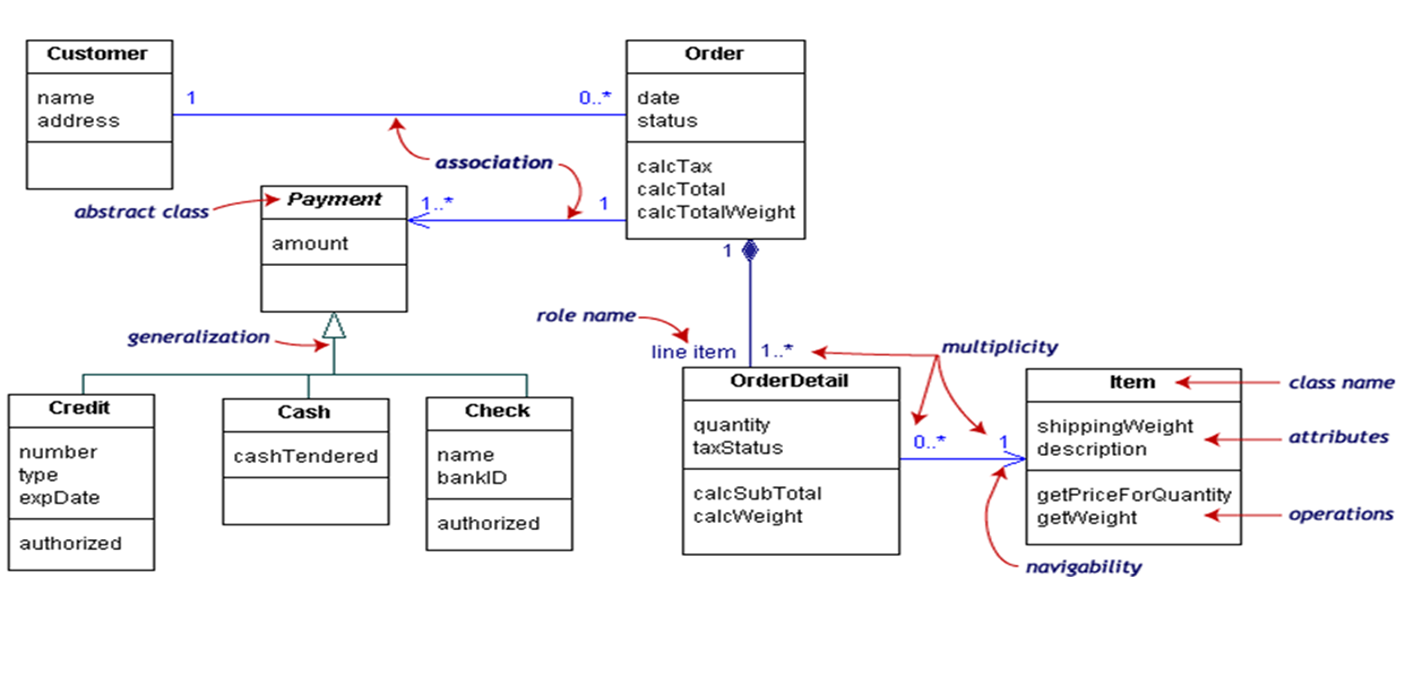
\includegraphics[width=0.9\linewidth]{class.png}
    \caption{Caption}
    \label{fig:enter-label}
\end{figure}
\subsection{Sequence Diagram}
Add description and diagram

\subsection{State Transition Diagram }
Add description and diagram

\section{Data Design}
Explain how the information domain of your system is transformed into data structures. Describe how the major data or system entities are stored, processed, and organized. 

List any databases or data storage items.

\subsection{Data Dictionary}
Alphabetically list the system entities or major data along with their types and descriptions. If you provided a functional description, list all the functions and function parameters. If you provided an OO description, list the objects and its attributes, methods and method parameters. 

\section{Human Interface Design}
Describe the functionality of the system from the user’s perspective. Explain how the user will be able to use your system to complete all the expected features and the feedback information that will be displayed for the user.

\subsection{Screen Images} 
Display screenshots showing the interface from the user’s perspective. These can be hand-drawn, or you can use an automated drawing tool. Just make them as accurate as possible. (Graph paper works well.) 

\subsection{Screen Objects and Actions}
A discussion of screen objects and actions associated with those objects.


\section{Algorithm}
Mention the algorithm(s) used in your project to get the work done with regards to major modules. Provide a pseudocode explanation regarding the functioning of the core features. Be sure to use the correct syntax and semantics for algorithm representations. Following are few examples of algorithms/pseudocode:


\section{Tools and Technologies}
Mention all the hardware/software tools and technologies with version number which will be used in implementation of the project. Write about the APIs, language(s), SDK(s) etc. which you will use for implementation. 

\begin{table}[h]
\centering
\caption{Tools and Technologies for Proposed Project}
\begin{tabular}{|c|p{3.5cm}|p{3.5cm}|p{3.5cm}|}
\hline
\multirow{8}{*}{\textbf{Tools and Technologies}} & \textbf{Tool} & \textbf{Version} & \textbf{Rationale} \\ \cline{2-4}
& & & \\ \cline{2-4}
& & & \\ \cline{2-4}
& & & \\ \cline{2-4}
& & & \\ \cline{2-4}
& & & \\ \cline{2-4}
& & & \\ \cline{2-4}
& & & \\ \hline
\end{tabular}
\end{table}


\section{External APIs/SDKs}
Describe the third-party APIs/SDKs used in the project implementation in the following table. Few examples of APIs are provided in the table.

\section{User Interface}
Details about user interface with descriptions. Provide the User Interface for each sub-system (such as Mobile App, Web App, Client App, Admin App). Provide description of each User Interface explaining the details.
When inserting User Interfaces, use appropriate size of the image, for example, for mobile app, 2-4 screens can be placed on a single page.

Following are few examples of User Interfaces:

\subsection{Login and Home screen}
Login screen of our mobile app where user have to choose its role and its company.
Home screen where total, delayed and other complaints are shown. \ref{screen1}

\begin{figure}[h]
	\centering
	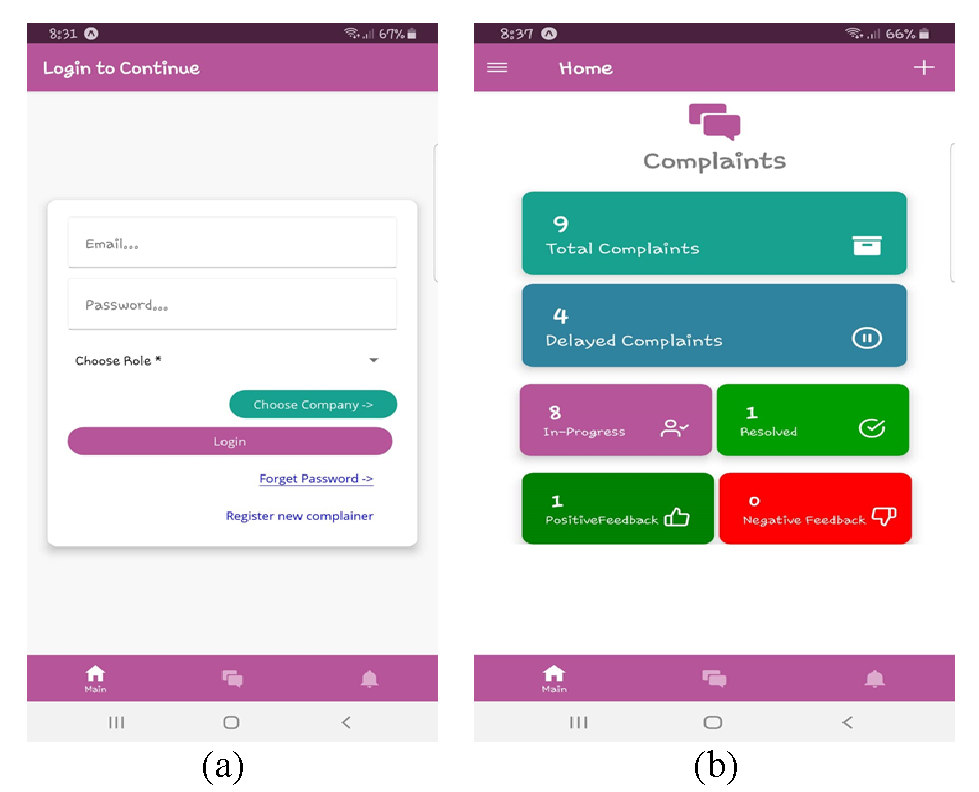
\includegraphics[width=0.7\textwidth]{screen.pdf}
	\caption{A screen shows interface a)login screen and b) menu screen.}
	\label{screen1}
\end{figure} 
\newpage
\subsection{Assignee Dashboard}
Complain Assignee can view the graphs of month-wise complains, Resolved complains, summary and a list of submitted complains \ref{screen2}.

\begin{figure}[h]
	\centering
	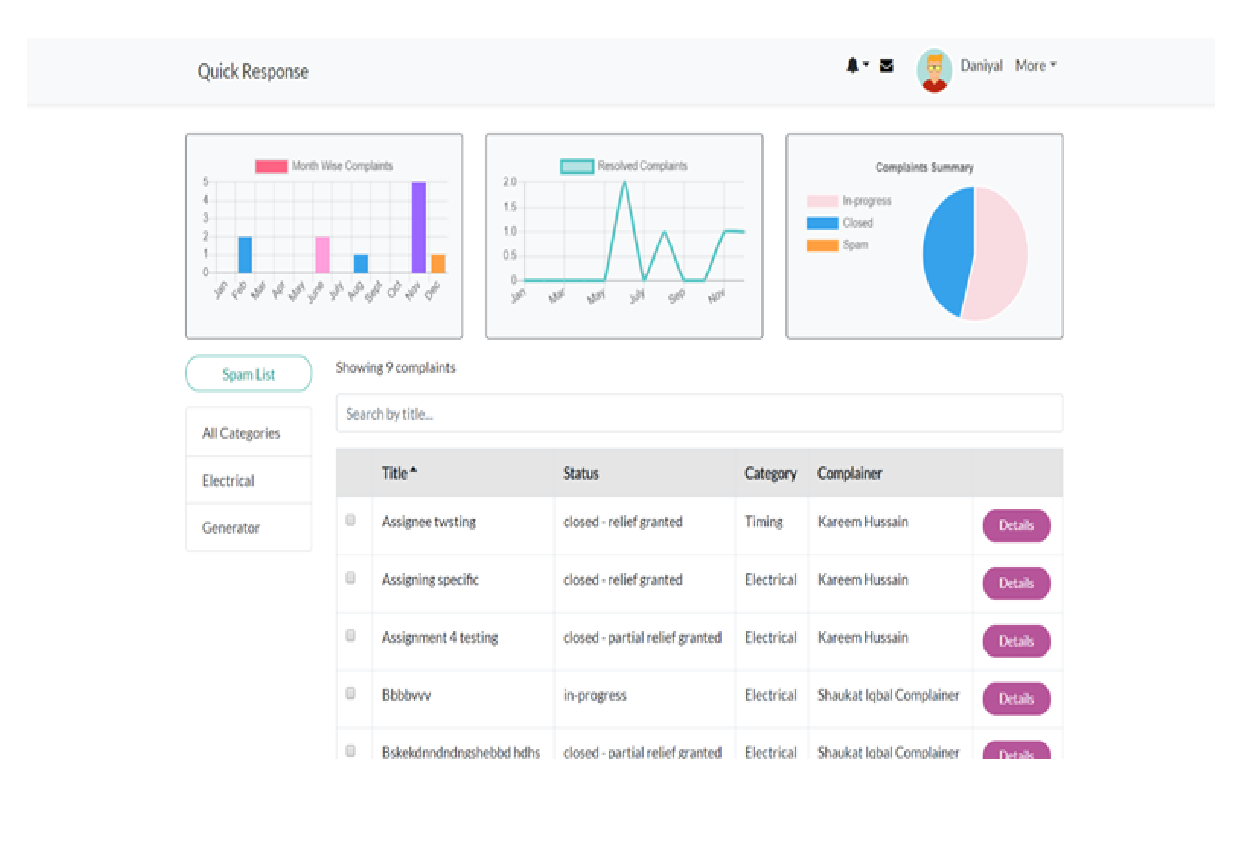
\includegraphics[width=0.5\textwidth]{screen_2.pdf}
	\caption{A screen shows interface of Assignee Dashboard}
	\label{screen2}
\end{figure} 

\section{Deployment}
Specify the deployment environments used for hosting and live testing of all the sub-systems of the project. Provide the details of hosting/cloud service used, set of available software and their versions used etc.

\begin{figure}[h]
	\centering
	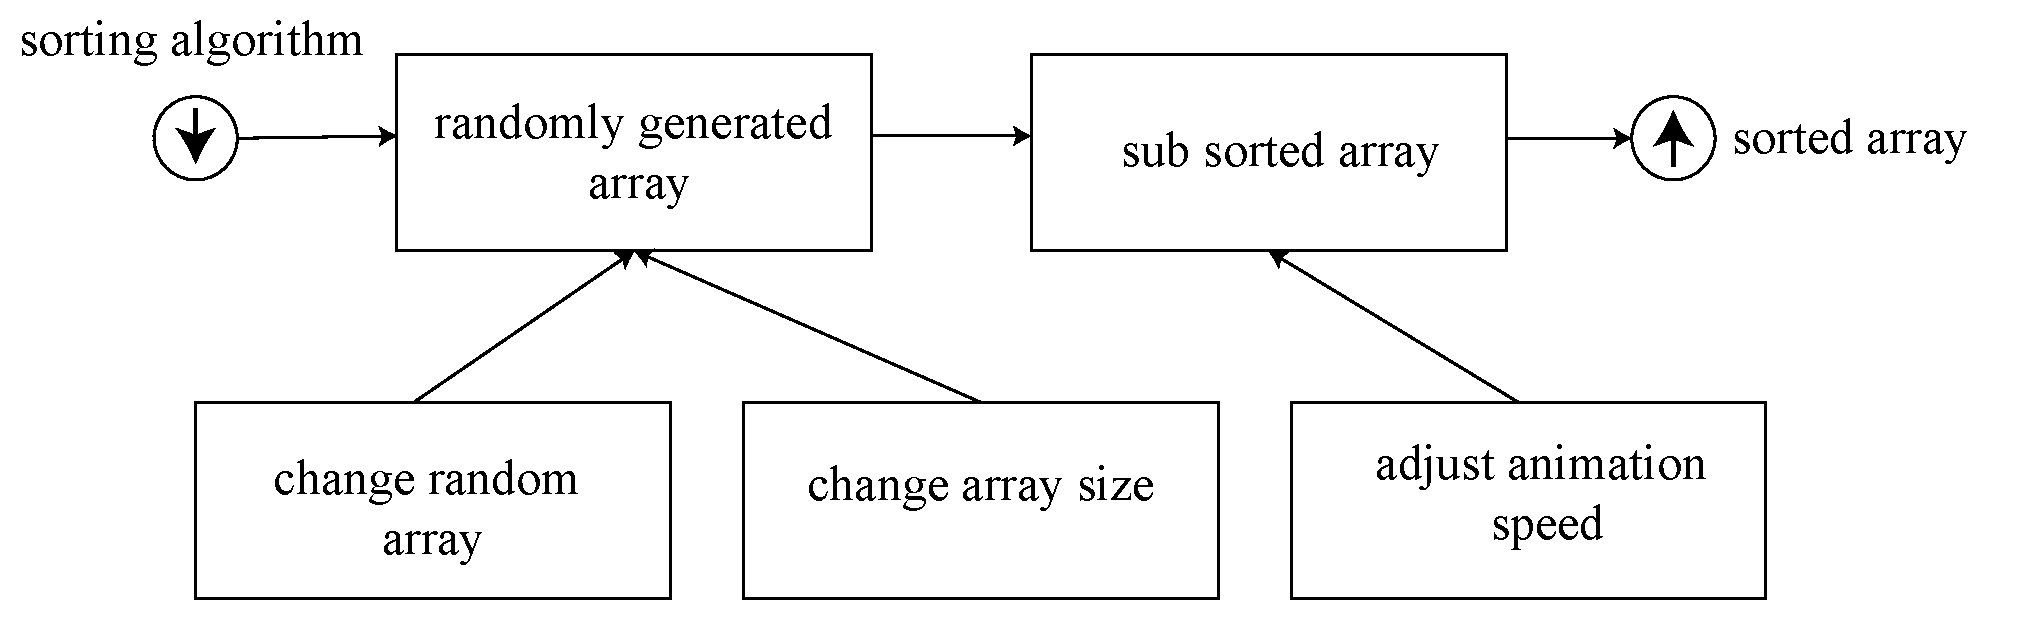
\includegraphics[width=0.5\linewidth]{architecture.pdf}
	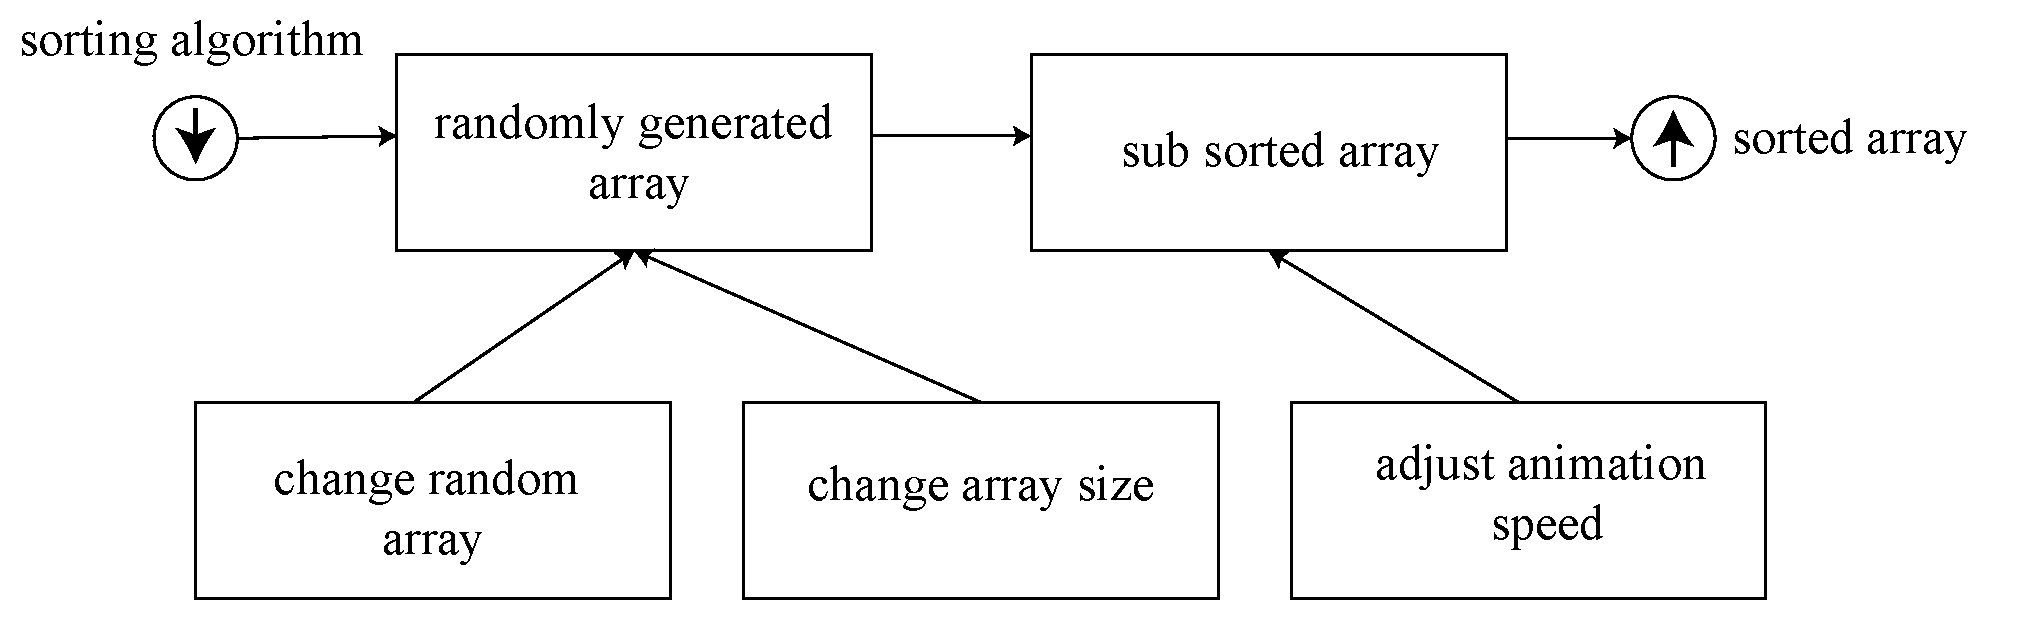
\includegraphics[width=0.5\linewidth]{architecture.pdf}
	\caption{An example of presenting multiple images in one figure, top is arch 1 and bottom is arch 2}
	\label{screen3}
\end{figure} 

\begin{figure}[h]
	\centering
	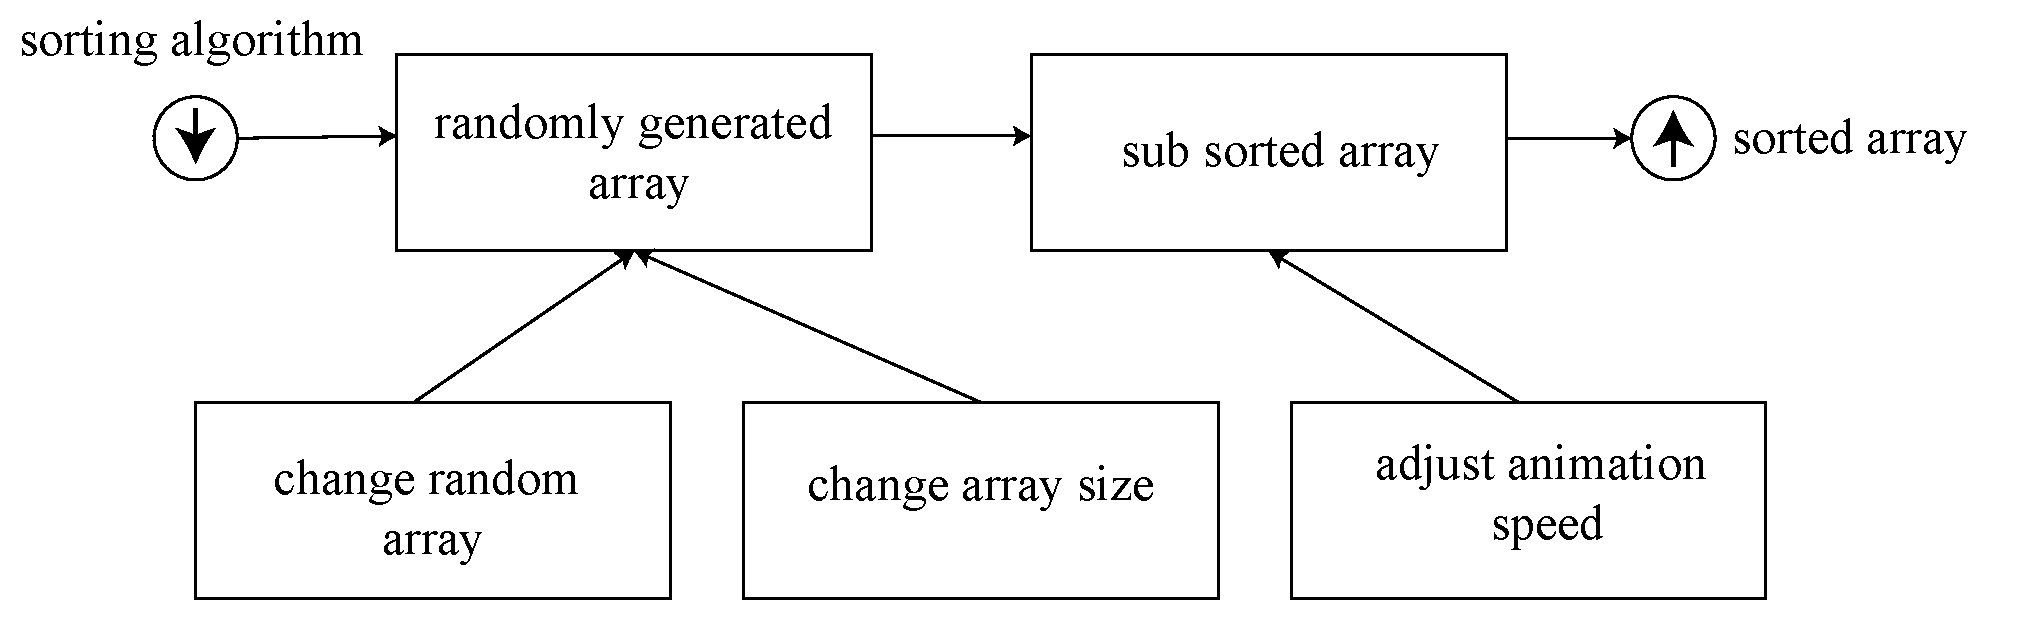
\includegraphics[width=.45\linewidth]{architecture.pdf}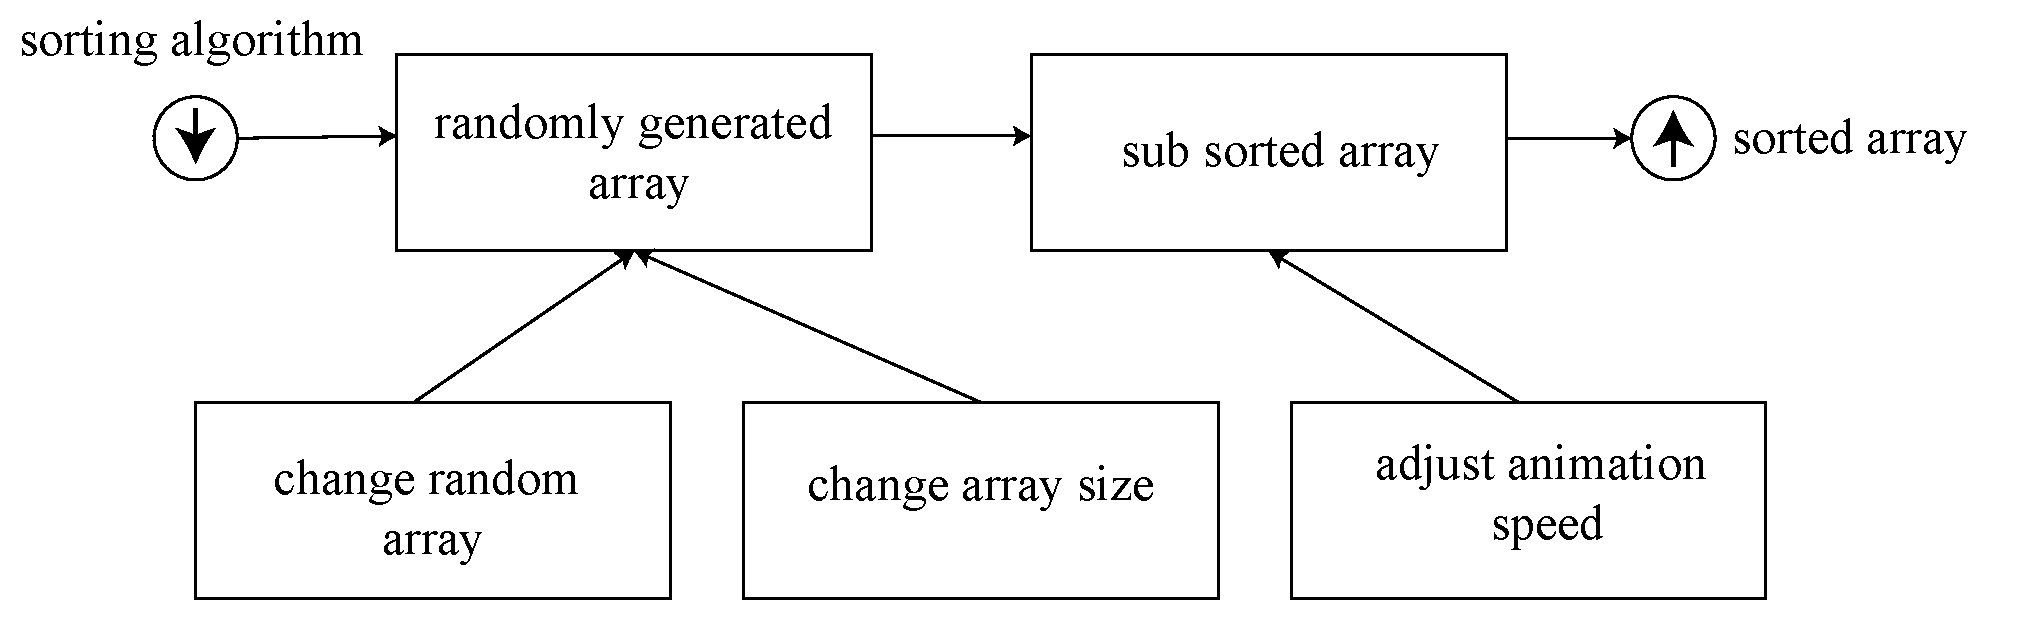
\includegraphics[width=.45\linewidth]{architecture.pdf}	
	\caption{An example of presenting multiple images in one figure, left is arch 1 and right is arch 2}
	\label{screen4}
\end{figure} 

\begin{figure}[h]
	\centering
	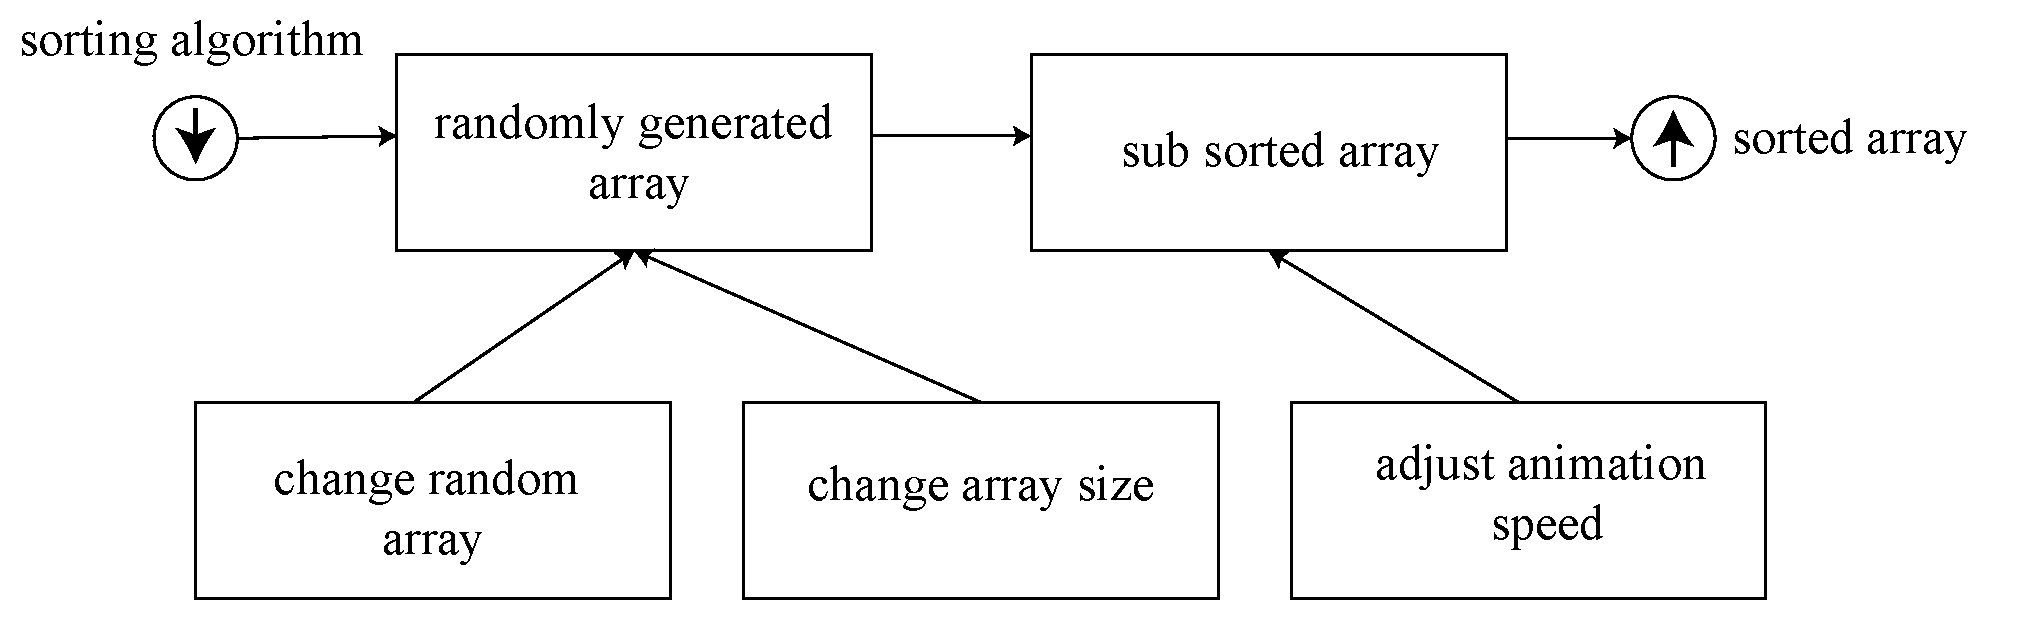
\includegraphics[width=.45\linewidth]{architecture.pdf}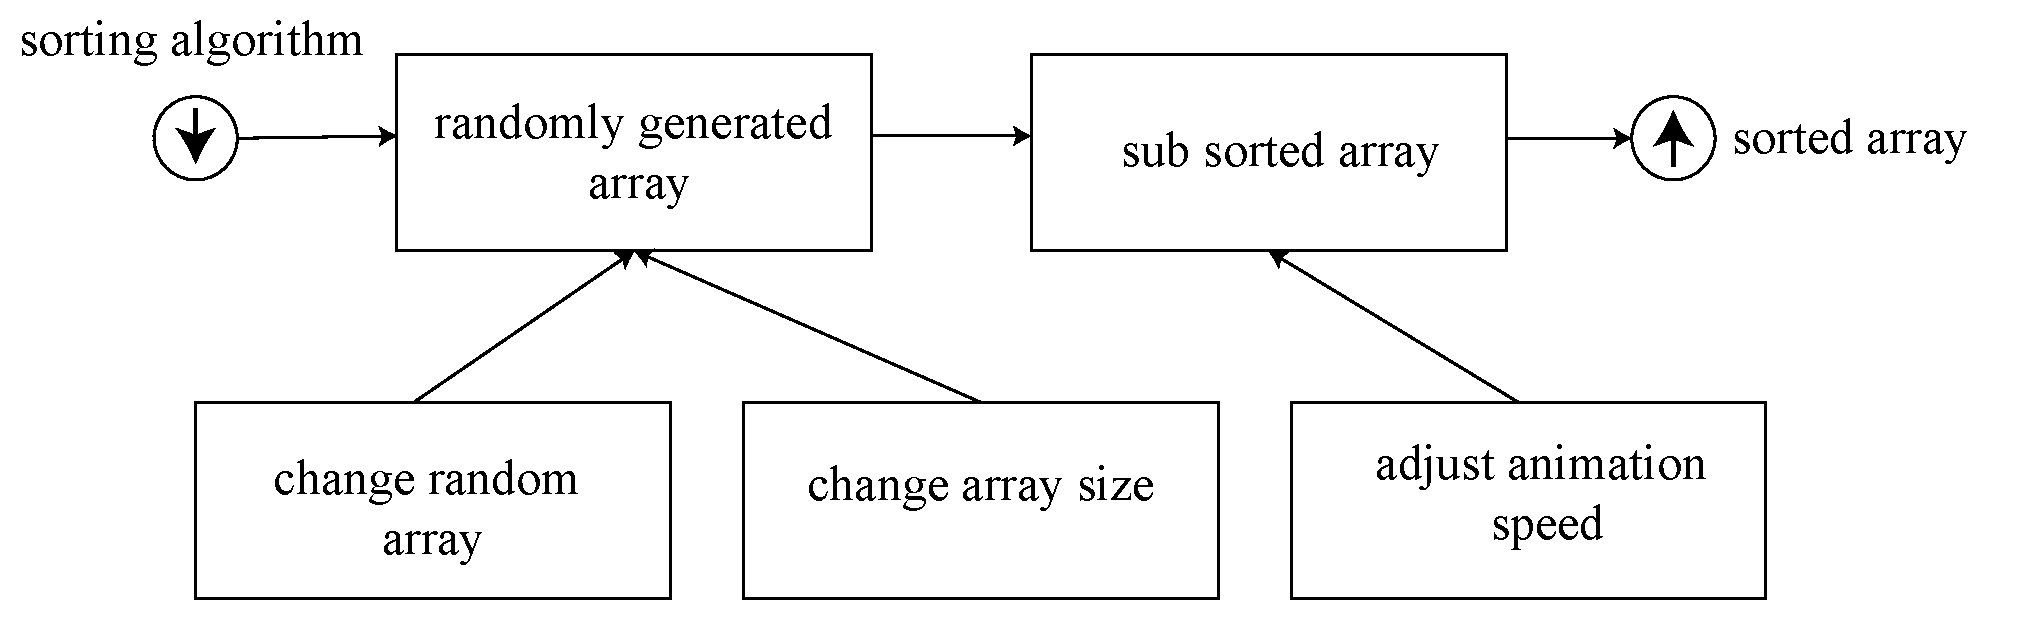
\includegraphics[width=.45\linewidth]{architecture.pdf}	
	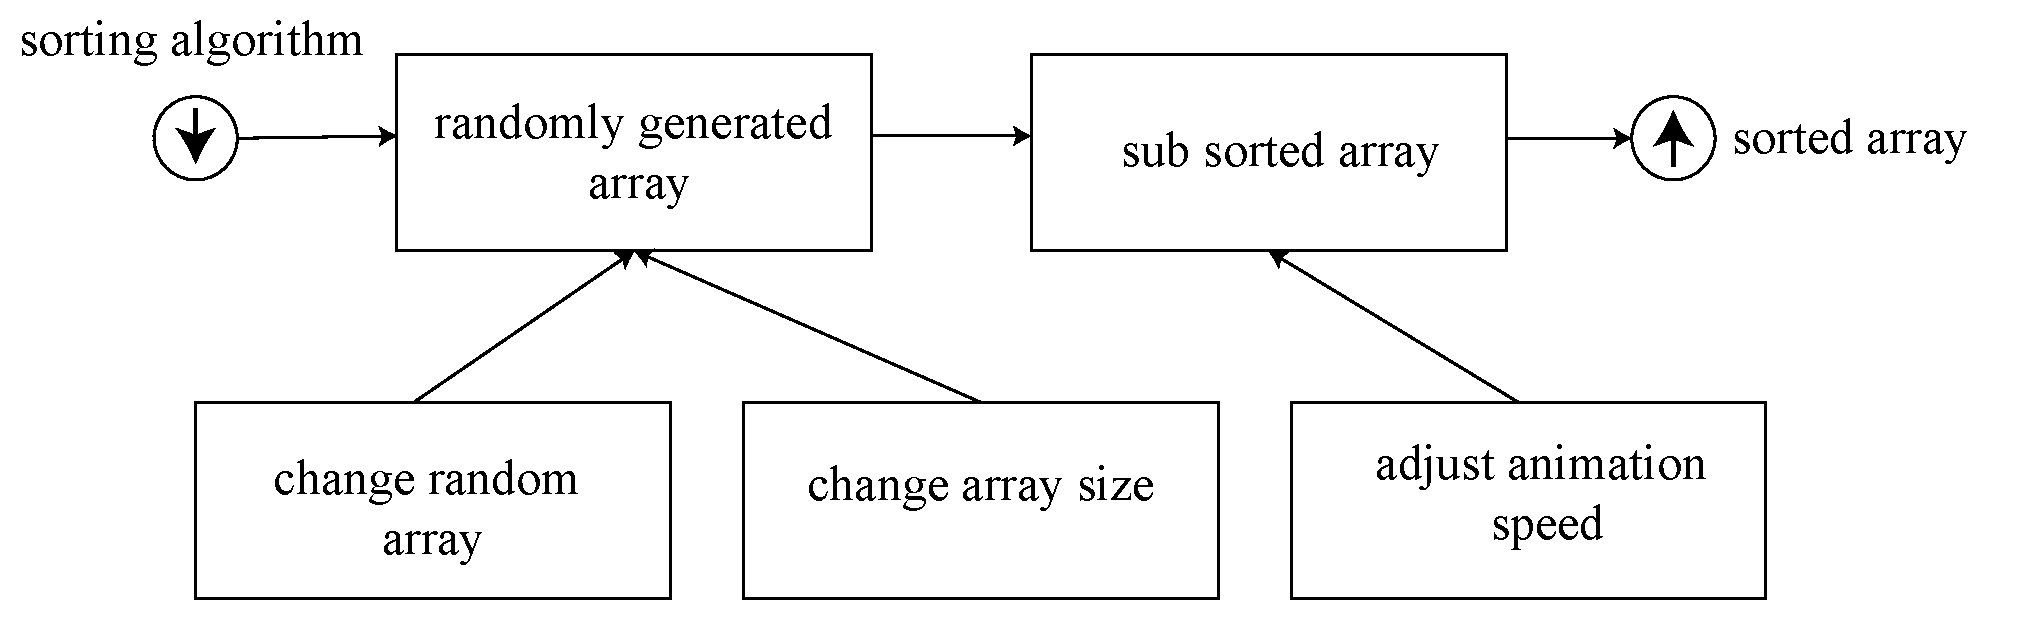
\includegraphics[width=.45\linewidth]{architecture.pdf}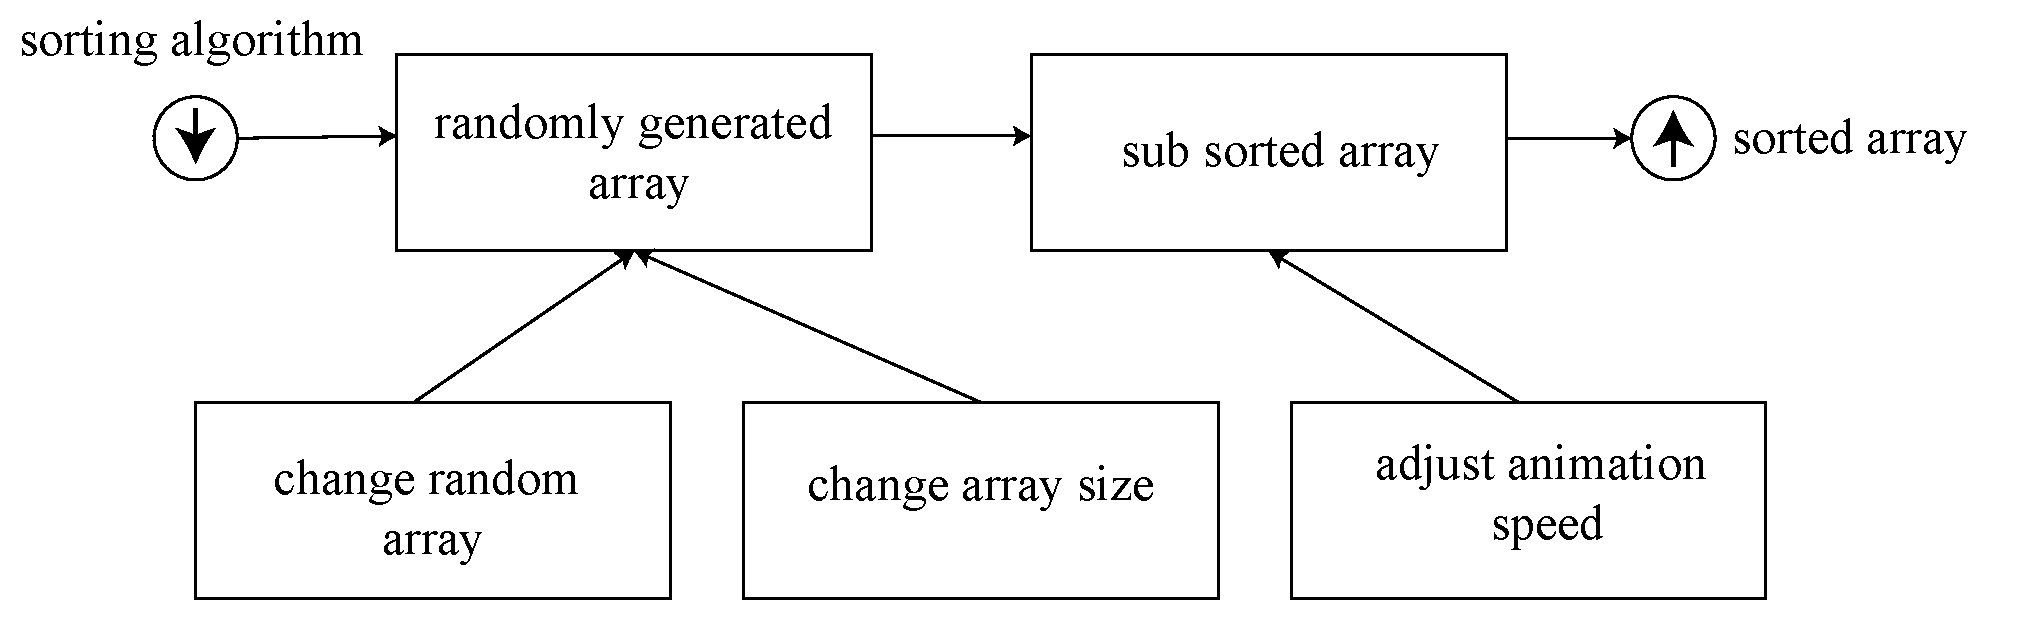
\includegraphics[width=.45\linewidth]{architecture.pdf}	
	\caption{An example of presenting multiple images in one figure, use labels A, B, C, D}
	\label{screen5}
\end{figure}

\begin{table}[h]
	\centering
	\caption{an example of multi column table}
	\begin{tabular}[c]{|p{3cm}|p{3cm}|p{3cm}|p{3cm}|}
		\toprule
		\multicolumn{2}{c}{combine columns} & \multicolumn{2}{c}{combine columns} \\
		\midrule
		x&y&x&y\\
		\midrule
		1&2&3&4\\

		1&2&3&4\\

		1&2&3&4\\
		\bottomrule
	\end{tabular}
\end{table}

\begin{table}[h]
	\centering
	\caption{bullets and numbering in a table}
	\begin{tabular}[c]{|p{3cm}|p{3cm}|p{3cm}|p{3cm}|}
		\toprule
		columns 1 & columns 2 & columns 3 & columns 4 \\
		\midrule
		\begin{itemize}[leftmargin=10px]
			\item point 1
			\item point 2
		\end{itemize}&
		\begin{enumerate}[leftmargin=10px]
		\item point 1
		\item point 2
		\end{enumerate}&x&y\\
		\midrule
		1&2&3&4\\
		
		1&2&3&4\\
		
		1&2&3&4\\
		\bottomrule
	\end{tabular}
\end{table}
\section{Chapter Summary}
Chapter summary comes here


\chapter{Testing and Evaluation}
\thispagestyle{empty}
\newpage
\begin{spacing}{1.5}
\pagenumbering{arabic}

\thispagestyle{empty}

% --- Centered chapter title, same size as normal chapter ---
{\centering \Large \bfseries Chapter Overview \par}
\vspace{1cm} % adjust space after title

% --- Chapter introduction text (not numbered) ---
This chapter introduces the background, motivation, and problem
statement of the project. It highlights the research gap and explains
why this study is important. The chapter also outlines the objectives
and structure of the work.

\end{spacing}

\section{Unit Testing}

It’s a level of software testing where individual units of a software/component are tested. The purpose is to validate that each unit of the software performs as designed.

Unit Testing 1:   Login as Patient with valid and invalid credentials

Testing Objective: To ensure the login form is working correctly with valid and invalid credentials/inputs.

\section{Functional Testing}
The functional testing will take place after the unit testing. In this functional testing, the functionality of each of the module is tested. This is to ensure that the system produced meets the specifications and requirements.

Functional Testing 1: Login with different roles (Management, Patient, Doctor) 

Objective: To ensure that the correct page with the correct navigation bar is loaded.  

\section{Business Rules Testing}
Decision table based testing technique is used to test business rules. The business rules were defined in FRs and Use Cases
Decision based testing uses a systematic approach where input and outputs are provided in tabular form. It is a precise and compact way to model complicated logic. The table contains conditions and actions are used for test cases where conditions as inputs and actions as outputs.

Detailed example is as given in Appendix E. see reference \cite{Abuleil2023}

\section{Integration Testing}
Integration tests assess whether a set of classes that must work together do so without error. They
ensure that the interfaces and linkages between different parts of the system work properly. At this point, the classes have passed their individual unit tests, so the focus now is on the flow of control among the classes and on the data exchanged among them. Integration testing follows the same general procedures as unit testing: The tester develops a test plan that has a series of tests, which, in turn, have a test. Integration testing is often done by a set of programmers and/or systems analysts.

Integration Testing 1:   Scheduling Patient Appointment

Testing Objective: To ensure the scheduling is being done correctly and the interface between module ‘Patient/Doctor Management’ and module ‘Appointment/Scheduling’ is running correctly.
\section{Chapter Sumamry}
chapter summary goes here


\newpage

\chapter{Conclusion and future work}
\thispagestyle{empty}
\newpage
\begin{spacing}{1.5}
\pagenumbering{arabic}

\thispagestyle{empty}

% --- Centered chapter title, same size as normal chapter ---
{\centering \Large \bfseries Chapter Overview \par}
\vspace{1cm} % adjust space after title

% --- Chapter introduction text (not numbered) ---
This chapter introduces the background, motivation, and problem
statement of the project. It highlights the research gap and explains
why this study is important. The chapter also outlines the objectives
and structure of the work.



\section{Conclusion}
This chapter summarizes the major contributions and findings of this project. The primary objective of this work was to design and develop an automated spot-specific spraying system for weed detection in wheat crops. The proposed approach successfully achieved this objective by combining machine learning techniques with image processing to detect and localize weeds in real time.

The results demonstrated that the proposed system was able to
accurately identify weed-infested regions and perform precise
spot-specific spraying. The outcomes confirmed that the methodology
reduced unnecessary pesticide usage while maintaining effectiveness.
The findings highlight the significance of this work in promoting
sustainable agriculture by reducing chemical consumption, lowering
costs, and minimizing environmental impact.

\section{Future Work}
Although the project achieved its intended objectives, there are
several directions for future research and improvement:

\begin{itemize}
    \item \textbf{Dataset Expansion:} Incorporate a larger and more
    diverse dataset covering different crop growth stages, weed types,
    and field conditions.
    
    \item \textbf{Model Enhancement:} Explore advanced deep learning
    architectures, such as transformers or reinforcement learning,
    to improve detection accuracy and decision-making.
    
    \item \textbf{Hardware Optimization:} Implement more efficient
    spraying mechanisms and integrate lightweight hardware for
    real-time field deployment.
    
    \item \textbf{Scalability:} Extend the system for other crops
    beyond wheat, and test it in large-scale farming scenarios.
    
    \item \textbf{Integration with Smart Agriculture:} Combine the
    spraying system with IoT sensors, drones, or autonomous ground
    robots for fully automated precision farming solutions.
\end{itemize}

In conclusion, while the proposed system provides a strong foundation
for automated weed management, future enhancements will enable more
robust, scalable, and intelligent solutions for precision agriculture.
\section{Chapter Summary}

\end{spacing}
\chapter*{References}
\addcontentsline{toc}{chapter}{References}

\begin{thebibliography}{1}
%\addcontentsline{toc}{chapter}{References}
%\thispagestyle{empty}
%\newpage
\vspace{-6cm}
\bibitem{1} C. Shen, S. Yu, J. Wang, G. Q. Huang, and L. Wang, “A Comprehensive Survey on Deep Gait Recognition: Algorithms, Datasets and Challenges,” 2022, doi: 10.48550/ARXIV.2206.13732. 

\bibitem{2} J. Han and B. Bhanu, “Individual recognition using gait energy image,” IEEE Trans. Pattern Anal. Mach. Intell., vol. 28, no. 2, pp. 316–322, Feb. 2006, doi: 10.1109/TPAMI.2006.38. 

\bibitem{3} H. Iwama, M. Okumura, Y. Makihara, and Y. Yagi, “The OU-ISIR Gait Database Comprising the Large Population Dataset and Performance Evaluation of Gait Recognition,” IEEE Trans. Inf. Forensics Secur., vol. 7, no. 5, pp. 1511–1521, Oct. 2012, doi: 10.1109/TIFS.2012.2204253. 

\bibitem{data}  Shuai Zheng, Junge Zhang, Kaiqi Huang, Ran He and Tieniu Tan. Robust View Transformation Model for Gait Recognition. Proceedings of the IEEE International Conference on Image Processing, 2011

\bibitem{4} M. Bukhari et al., “An Efficient Gait Recognition Method for Known and Unknown Covariate Conditions,” IEEE Access, vol. 9, pp. 6465–6477, 2021, doi: 10.1109/ACCESS.2020.3047266. 

\bibitem{5} K. Bashir, T. Xiang, and S. Gong, “Cross View Gait Recognition Using Correlation Strength,” in Procedings of the British Machine Vision Conference 2010, Aberystwyth, 2010, p. 109.1-109.11. doi: 10.5244/C.24.109. 

\bibitem{6} R. Martín-Félez and T. Xiang, “Uncooperative gait recognition by learning to rank,” Pattern Recognit., vol. 47, no. 12, pp. 3793–3806, Dec. 2014, doi: 10.1016/j.patcog.2014.06.010. 

\bibitem{7} Xuelong Li, S. Lin, Shuicheng Yan, and Dong Xu, “Discriminant Locally Linear Embedding With High-Order Tensor Data,” IEEE Trans. Syst. Man Cybern. Part B Cybern., vol. 38, no. 2, pp. 342–352, Apr. 2008, doi: 10.1109/TSMCB.2007.911536. 

\bibitem{8} Dong Xu, Shuicheng Yan, Dacheng Tao, Lei Zhang, Xuelong Li, and Hong-Jiang Zhang, “Human Gait Recognition With Matrix Representation,” IEEE Trans. Circuits Syst. Video Technol., vol. 16, no. 7, pp. 896–903, Jul. 2006, doi: 10.1109/TCSVT.2006.877418. 

\bibitem{9} D. Tao, X. Li, X. Wu, and S. J. Maybank, “General Tensor Discriminant Analysis and Gabor Features for Gait Recognition,” IEEE Trans. Pattern Anal. Mach. Intell., vol. 29, no. 10, pp. 1700–1715, Oct. 2007, doi: 10.1109/TPAMI.2007.1096. 

\bibitem{10} H. Lee, S. Hong, and E. Kim, “An Efficient Gait Recognition with Backpack Removal,” EURASIP J. Adv. Signal Process., vol. 2009, no. 1, p. 384384, Dec. 2009, doi: 10.1155/2009/384384. 

\bibitem{11} K. Shiraga, Y. Makihara, D. Muramatsu, T. Echigo, and Y. Yagi, “GEINet: View-invariant gait recognition using a convolutional neural network,” in 2016 International Conference on Biometrics (ICB), Halmstad, Sweden, Jun. 2016, pp. 1–8. doi: 10.1109/ICB.2016.7550060. 

\bibitem{12} H. Chao, K. Wang, Y. He, J. Zhang, and J. Feng, “GaitSet: Cross-view Gait Recognition through Utilizing Gait as a Deep Set,” IEEE Trans. Pattern Anal. Mach. Intell., pp. 1–1, 2021, doi: 10.1109/TPAMI.2021.3057879. 

\bibitem{13} Z. Wu, Y. Huang, L. Wang, X. Wang, and T. Tan, “A Comprehensive Study on Cross-View Gait Based Human Identification with Deep CNNs,” IEEE Trans. Pattern Anal. Mach. Intell., vol. 39, no. 2, pp. 209–226, Feb. 2017, doi: 10.1109/TPAMI.2016.2545669. 

\bibitem{14} C. Fan et al., “GaitPart: Temporal Part-Based Model for Gait Recognition,” in 2020 IEEE/CVF Conference on Computer Vision and Pattern Recognition (CVPR), Seattle, WA, USA, Jun. 2020, pp. 14213–14221. doi: 10.1109/CVPR42600hing invariant human gait recognition using modified local optimal oriented pattern binary descriptor. Multimed Tools Appl 79, 2873–2896 (2020), doi: 10.1007/s11042-019-08400-8





\end{thebibliography}

\end{document}


